% !TEX encoding = UTF-8
\documentclass[xcolor=dvipsnames]{beamer}

\usepackage{lmodern}
\usepackage[ngerman]{babel}
\usepackage[utf8]{inputenc}
\usepackage{color}
\usepackage{graphicx}

\usetheme{CambridgeUS}
\usecolortheme{seahorse}
\useinnertheme{rectangles}
\setbeamertemplate{blocks}[rounded][shadow=false]



\beamertemplatenavigationsymbolsempty



\title{{\scriptsize{MA2STT2004 - Projektmodul\newline
\\\emph{Praxis der Digital Humanities}
\\Prof. Dr. Caroline Sporleder}}
\newline\\\textcolor{black}{\huge{Projektgruppe 2\newline
}}}
\author{C. Ahrens, A. Beyer, C. Michels}
\institute{Fachbereich II --  Computerlinguistik und Digital Humanities
\newline\\Universität Trier}
\date{\today}
%\logo{\includegraphics[scale=0.14]{logo-SF}}



\begin{document}

\begin{frame}[plain]
\titlepage
\end{frame}

\title{Projektgruppe 2}
\institute{}

\begin{frame}[plain]\frametitle{\textcolor{black}{Übersicht}}
\tableofcontents[hideallsubsections]
\end{frame}

%###########################################################################
%%%%%%%%%%%%%%%%%%%%%%%%%%%%%%%%%%%%%%%%%%%%%%%%%%%%%%%%
%###########################################################################

\section{Ansätze zur Koreferenzresolution}

%###########################################################################

\subsection{Barth}

%---

\begin{frame}[plain]\frametitle{\textcolor{black}{Übersicht}}

\tableofcontents[currentsection, hideothersubsections]

\end{frame}

\addtocounter{framenumber}{-3}

%---

\begin{frame}\frametitle{\textcolor{black}{Was ist Barth 2.0?}}

\begin{block}{Barth}
\begin{itemize}
\item Barth
\begin{itemize}
\item Barth
\end{itemize}
\item Barth
\item Barth
\end{itemize}
\end{block}

\end{frame}

%###########################################################################

\subsection{Reconcile}
%--- 

\begin{frame}\frametitle{\textcolor{black}{Was ist Reconcile?}}

\begin{block}{Reconcile}
\begin{itemize}
\item Reconcile
\begin{itemize}
\item Reconcile
\end{itemize}
\item Reconcile
\item Reconcile
\end{itemize}
\end{block}

\end{frame}

%###########################################################################

\subsection{DCoref}
%--- 

\begin{frame}\frametitle{\textcolor{black}{Was ist DCoref?}}

\begin{block}{DCoref}
\begin{itemize}
\item deterministisches Modul der Stanford CoreNLP
\begin{itemize}
\item hängt von anderen Modulen ab (pos, lemma, ner, parse)
\item diese Module müssen in der Pipeline vorher angewendet werden
\end{itemize}
\item arbeitet mit Sieben
\begin{itemize}
\item erste Stufe: bevorzugt Recall (detection)
\item zweite Stufe: Siebe bevorzugen Precision
\end{itemize} 
\item Post-Processing: mehr Precision (?)
\end{itemize}
\end{block}

\end{frame}

%###########################################################################
%%%%%%%%%%%%%%%%%%%%%%%%%%%%%%%%%%%%%%%%%%%%%%%%%%%%%%%%
%###########################################################################

\section{Verlauf}

%###########################################################################

\subsection{Vergleichen}

%---

\begin{frame}[plain]\frametitle{\textcolor{black}{Übersicht}}

\tableofcontents[currentsection, hideothersubsections]

\end{frame}

\addtocounter{framenumber}{-1}

%--- 

\begin{frame}\frametitle{\textcolor{black}{Suche nach dem besten Ansatz}}

\begin{block}{Vergleichsgegenstände}
\begin{itemize}
\item Reconcile
\item DCoref
\end{itemize}
\end{block}

\begin{block}{Vergleichspunkte}
\begin{itemize}
\item Precision
\item Recall
\item FScore
\end{itemize}
\end{block}

\end{frame}

%--- 

\begin{frame}\frametitle{\textcolor{black}{Suche nach dem besten Ansatz}}

\begin{block}{Werkzeug: MMAX}
\begin{itemize}
\item Schwierigkeiten bei der Verwendung
\begin{itemize}
\item Vergleich war entsprechend auch schwierig
\end{itemize}
\end{itemize}
\end{block}

\begin{block}{Testdaten: Uncle Tom's Cabin}
\begin{itemize}
\item erste Hälfte des ersten Kapitels, Reintext
\begin{itemize}
\item bis zu dem Wort \emph{Wilberforce}
\item eindeutige Grenze
\end{itemize}
\end{itemize}
\end{block}

\end{frame}

%--- 

\begin{frame}\frametitle{\textcolor{black}{``{Version Space (Angepasst)}''. \emph{Wikimedia Commons}.}}
\begin{figure}
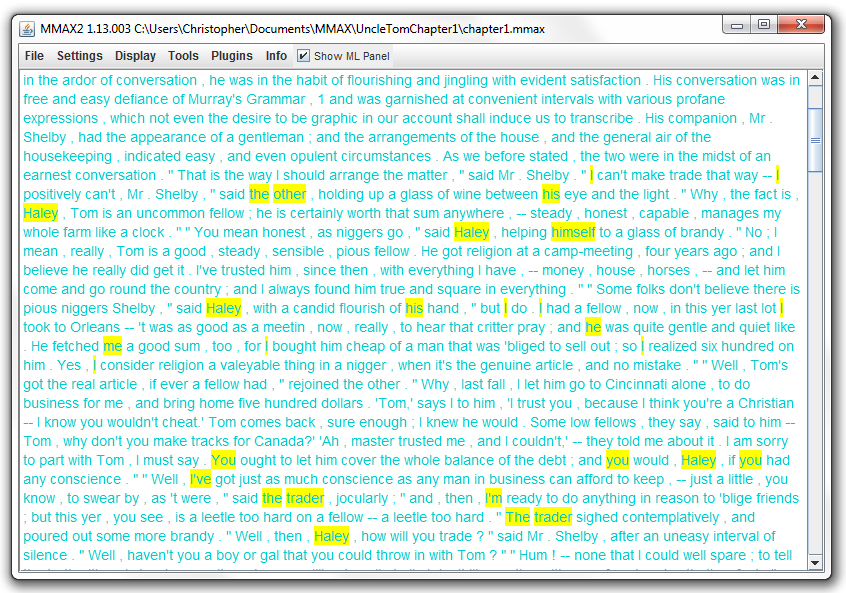
\includegraphics[height=7cm]{cm_mmax.jpg}
\end{figure}

\end{frame}

%###########################################################################


\subsection{Formatieren}

%---

\begin{frame}\frametitle{\textcolor{black}{Formatieren: Reconcile}}

\begin{block}{Reconcile}
\begin{itemize}
\item Formatieren
\begin{itemize}
\item Formatieren
\item Formatieren
\end{itemize}
\end{itemize}
\end{block}

\end{frame}

%---

\begin{frame}\frametitle{\textcolor{black}{Formatieren: DCoref}}

\begin{block}{DCoref}
\begin{itemize}
\item Formatieren
\begin{itemize}
\item Formatieren
\item Formatieren
\end{itemize}
\end{itemize}
\end{block}

\end{frame}

%###########################################################################


\subsection{Indizieren}

%---

\begin{frame}\frametitle{\textcolor{black}{Indizieren: Reconcile}}

\begin{block}{Indizieren}
\begin{itemize}
\item Indizieren
\begin{itemize}
\item Indizieren
\end{itemize}
\end{itemize}
\end{block}

\end{frame}

%---

\begin{frame}\frametitle{\textcolor{black}{Indizieren: DCoref}}

\begin{block}{Input}
\begin{itemize}
\item Indizieren
\begin{itemize}
\item Indizieren
\end{itemize}
\end{itemize}
\end{block}

\begin{block}{Output}
\begin{itemize}
\item Indizieren
\begin{itemize}
\item Indizieren
\end{itemize}
\end{itemize}
\end{block}

\end{frame}

%###########################################################################
%%%%%%%%%%%%%%%%%%%%%%%%%%%%%%%%%%%%%%%%%%%%%%%%%%%%%%%%
%###########################################################################

\section{Demonstration}

%###########################################################################

\subsection{Reconcile}

%---

\begin{frame}[plain]\frametitle{\textcolor{black}{Übersicht}}

\tableofcontents[currentsection, hideothersubsections]

\end{frame}

\addtocounter{framenumber}{-1}

%--- 

\begin{frame}\frametitle{\textcolor{black}{``{Version Space (Angepasst)}''. \emph{Wikimedia Commons}.}}
\begin{figure}
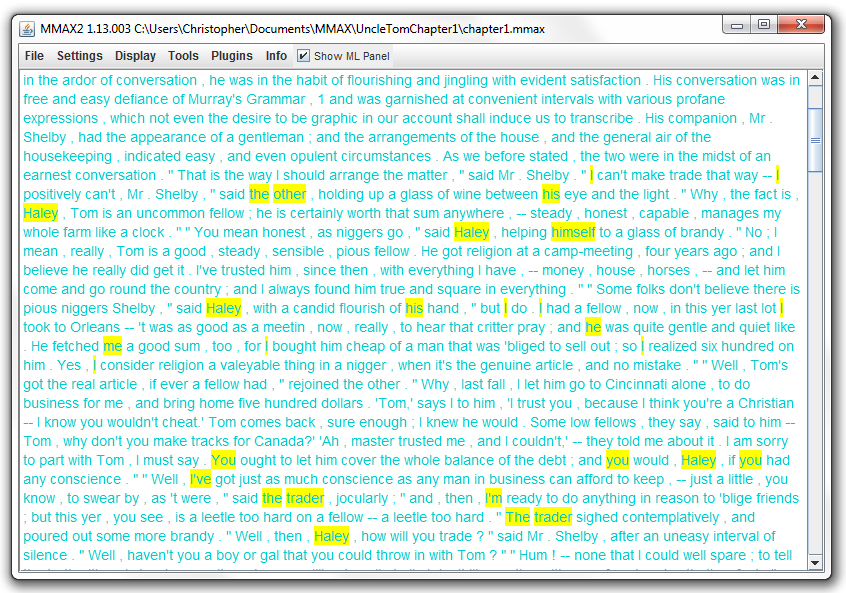
\includegraphics[height=7cm]{cm_mmax.jpg}
\end{figure}

\end{frame}

%###########################################################################

\subsection{DCoref}

%--- 

\begin{frame}\frametitle{\textcolor{black}{``{Version Space (Angepasst)}''. \emph{Wikimedia Commons}.}}
\begin{figure}
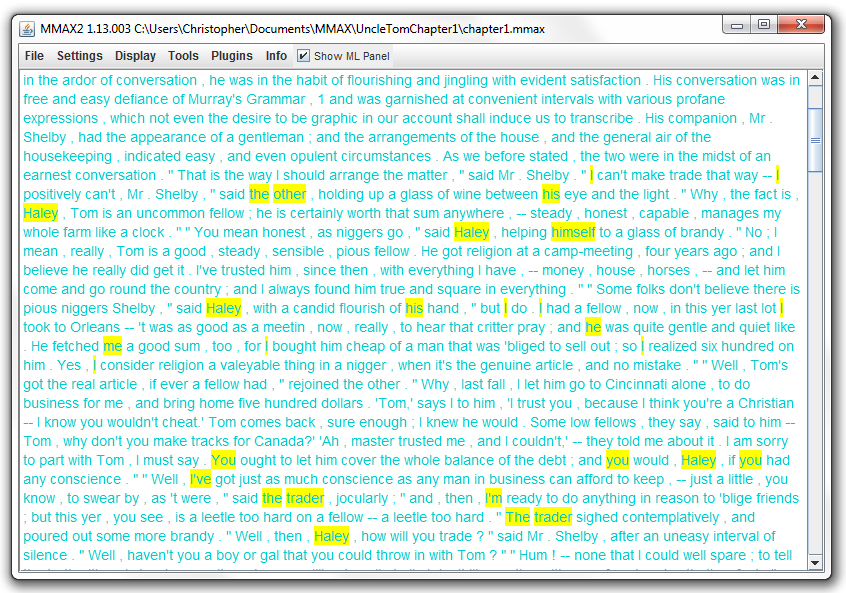
\includegraphics[height=7cm]{cm_mmax.jpg}
\end{figure}

\end{frame}

\addtocounter{framenumber}{-3}

%---

\begin{frame}[plain]
\frametitle{\textcolor{black}{Zeit für Fragen}}
Gibt es noch offene Fragen oder Dinge, die unklar geblieben sind?
\end{frame}

\begin{frame}[plain]
\frametitle{\textcolor{black}{Zum Schluss}}
Vielen Dank für eure Aufmerksamkeit!
\end{frame}

%\begin{frame}[plain]
%\frametitle{\textcolor{black}{Literatur}}
%\begin{thebibliography}{9}
%\bibitem[Mitchell]{buch} Mitchell, Tom M. (1982). ``Generalization as search". \emph{Artificial Intelligence} 18 (2): 203–226.
%\bibitem[Rendell]{buch} Rendell, Larry (1986). ``A general framework for induction and a study of selective induction". \emph{Machine Learning} 1 (2): 177–226.
%\bibitem[Sverdlik]{buch} Sverdlik, W.; Reynolds, R.G. (1992). ``Dynamic version spaces in machine learning". Proceedings, \emph{Fourth International Conference on Tools with Artificial Intelligence (TAI '92)}. Arlington, VA. pp. 308–315.
%\end{thebibliography}
%\end{frame}



\end{document}
